\documentclass[11pt,a4paper]{article}

% Typography and fonts
\usepackage[T1]{fontenc}
\usepackage{mathpazo}
\usepackage{microtype}

% Layout
\usepackage[margin=1in]{geometry}
\usepackage{setspace}
\onehalfspacing

% Graphics and diagrams
\usepackage{tikz}
\usetikzlibrary{positioning, arrows.meta, shapes.geometric, fit, calc, decorations.pathreplacing}

% Tables, lists, code
\usepackage{booktabs}
\usepackage{enumitem}
\usepackage{listings}
\usepackage{xcolor}

% Links and PDF metadata
\usepackage[hidelinks]{hyperref}
\usepackage{url}

% Math
\usepackage{amsmath,amssymb}

% Section styling
\usepackage{titlesec}
\titleformat{\section}{\Large\bfseries}{\thesection.}{0.5em}{}
\titleformat{\subsection}{\large\bfseries}{\thesubsection}{0.5em}{}
\titleformat{\subsubsection}{\normalsize\bfseries}{\thesubsubsection}{0.5em}{}

% Code listing style
\lstset{
  basicstyle=\ttfamily\small,
  breaklines=true,
  frame=single,
  backgroundcolor=\color{gray!5},
  keywordstyle=\color{blue!70!black},
  commentstyle=\color{green!50!black},
  stringstyle=\color{red!60!black},
}

% Custom colors
\definecolor{ekweblue}{RGB}{30,60,114}
\definecolor{ekwegold}{RGB}{180,140,20}

\begin{document}

% ============================================================
% TITLE PAGE
% ============================================================
\begin{titlepage}
\centering
\vspace*{2cm}

{\fontsize{14}{16}\selectfont\color{ekweblue}\textsc{Ekwe Technologies Limited}}

\vspace{1.5cm}

{\fontsize{28}{34}\selectfont\bfseries\color{ekweblue} Ekwe Protocol}

\vspace{0.5cm}

{\fontsize{14}{18}\selectfont\itshape A Decentralized Event-Driven Edge Network\\for Resilient Push Messaging and Offline Transactions\\Anchored to a Bitcoin Layer-2}

\vspace{2cm}

{\large David Nzagha}\\[0.3cm]
{\normalsize Ekwe Technologies Limited \quad$\cdot$\quad Nzagha Ventures Limited}

\vspace{1.5cm}

{\normalsize Version 1.0 \quad$\cdot$\quad February 2026}

\vspace{2cm}


\begin{tikzpicture}
  \draw[ekweblue, line width=2pt] (0,0) circle (1.2cm);
  \draw[ekwegold, line width=1.5pt] (0,0) circle (0.8cm);
  \node[font=\Large\bfseries, color=ekweblue] at (0,0) {E};
\end{tikzpicture}

\vfill

{\small\textit{``The ancestral drum of the future.\\A sovereign event-driven messaging network powered by people, proof, and Bitcoin.''}}

\vspace{1cm}
\end{titlepage}

% ============================================================
% ABSTRACT
% ============================================================
\newpage
\begin{abstract}
\noindent
Mission-critical services in regions with intermittent connectivity require reliable dissemination primitives that do not assume continuous Internet access or centralized operators. Contemporary push-notification infrastructures (Apple Push Notification service [APNs] and Firebase Cloud Messaging [FCM]) provide scalable targeted delivery but fundamentally depend on always-reachable cloud brokers and stable IP connectivity~\cite{apns}. Unstructured Supplementary Service Data (USSD) remains a dominant access channel for mobile financial services in African markets because it operates over cellular signaling channels without requiring an Internet data plan; however, USSD is session-bound to mobile network operator infrastructure, offers limited programmability, and fails under cellular outages~\cite{etsi_ussd_stage1}.

This paper specifies \textbf{Ekwe Protocol}, a decentralized, event-driven edge computing network designed for mission-critical operations in challenged environments. The protocol provides a ``push-like'' messaging substrate supporting offline-first delivery, multi-radio relaying (Bluetooth Low Energy, Wi-Fi peer-to-peer, LoRaWAN, and optional legacy radio), and programmable event execution with verifiable computation. Ekwe adopts an asynchronous message-and-fee model inspired by The Open Network (TON)~\cite{ton_whitepaper}, enabling per-event gas accounting and incentive-compatible reward splitting across relayers, executors, and chain committers. For global settlement and auditability, Ekwe targets a Bitcoin Layer-2 (L2) design using periodic commitments to Bitcoin, leveraging recent work on Bitcoin L2 design patterns~\cite{sok_btc_l2} and BitVM-style bridging~\cite{bitvm2}.

The paper contributes: (I)~a system model and protocol architecture for decentralized push delivery under disruption; (II)~a transport-agnostic event format and routing/relay logic tailored to store-and-forward edge networks; (III)~a TON-inspired gas and reward mechanism aligned with Decentralized Physical Infrastructure Networks (DePIN); (IV)~a dual-token economic model (\$EKWE utility token and BTC mining rewards); and (V)~an implementation and evaluation blueprint for the flagship offline-finance use case, EkwePay.
\end{abstract}

\vspace{0.5cm}
\noindent\textbf{Keywords:} Decentralized Physical Infrastructure Networks (DePIN), Delay/Disruption-Tolerant Networking (DTN), Push Notifications, USSD, LoRaWAN, Bluetooth Mesh, Wi-Fi Direct, Zero-Knowledge Proofs (ZKP), Verifiable Computing, Bitcoin Layer-2, Incentive Mechanisms, Edge Computing.

% ============================================================
% TABLE OF CONTENTS
% ============================================================
\newpage
\tableofcontents
\newpage

% ============================================================
% 1. INTRODUCTION & VISION
% ============================================================
\section{Introduction and Vision}

Digital public infrastructure increasingly assumes uninterrupted connectivity. In practice, connectivity is uneven, fragile, and frequently disrupted by power constraints, backhaul failures, congestion, or deliberate shutdowns. Under these conditions, critical operations (payments, medical logistics, emergency alerts, and safety coordination) degrade sharply when their communication substrate depends on centralized Internet services.

Push notification systems are a canonical example. APNs and FCM provide a standardized interface for applications to deliver targeted notifications to devices at global scale, but delivery requires a provider server to reach a centralized push service over the Internet~\cite{apns}. When connectivity is intermittent or absent, push delivery collapses into delayed polling, manual coordination, or complete silence.

USSD occupies a different niche. Defined for public land mobile networks (PLMNs) as a session-oriented mechanism enabling interactive exchanges between a mobile station and operator-defined applications via signaling channels~\cite{etsi_ussd_stage1}, USSD is widely used for mobile money and merchant transactions~\cite{gsma_ussd}. However, USSD is structurally constrained by the operator's signaling plane, limited message complexity, and the requirement of at least partial cellular service. It is therefore ``offline from the Internet,'' but not offline from the network.

\subsection{The Ekwe Drum: Cultural Foundation}

Ekwe Protocol is motivated by an older idea with modern constraints: the \textit{Ekwe}, a traditional communication drum used by Igbo communities in West Africa, as an always-on, community-scaled dissemination mechanism. The Ekwe drum served as a decentralized broadcast network: messages were encoded in tonal patterns, relayed across villages by drummers, and received by anyone within earshot. No central authority controlled the channel; any community member with an Ekwe could originate, relay, or respond to messages.

This ancestral model maps directly to the protocol's architecture:
\begin{itemize}[nosep]
  \item \textbf{Drummers} $\rightarrow$ \textbf{Relay Nodes}: community members who forward messages.
  \item \textbf{Drum patterns} $\rightarrow$ \textbf{Ekwe Events}: structured, signed message envelopes.
  \item \textbf{Village squares} $\rightarrow$ \textbf{Edge clusters}: local broadcast domains.
  \item \textbf{Inter-village relay chains} $\rightarrow$ \textbf{Multi-hop store-and-forward}: DTN-style propagation.
\end{itemize}

Ekwe Protocol aims to provide a decentralized, resilient, event-driven edge network that supports: (a)~push-like delivery without continuous Internet; (b)~local relaying by community-operated devices (including smartphones); (c)~programmable event execution at the edge; and (d)~cryptographic accountability and incentive alignment via a Bitcoin L2.

\subsection{Contributions}

The contributions of this paper are fivefold:
\begin{enumerate}[nosep]
  \item A system architecture for decentralized push-style dissemination over heterogeneous transports with store-and-forward semantics.
  \item A protocol-level event model supporting targeted delivery, scoped broadcast, subscription filtering, and replay resistance.
  \item A TON-inspired gas and reward splitting mechanism spanning forwarding, computation, and storage resources~\cite{ton_fees}.
  \item A dual-token economic model combining the \$EKWE utility token with Bitcoin mining rewards through dedicated hardware (EkweBox/Smartbox).
  \item An execution and settlement pipeline for verifiable event execution and delayed anchoring to Bitcoin L2~\cite{sok_btc_l2}.
\end{enumerate}

% ============================================================
% 2. BACKGROUND & MOTIVATION
% ============================================================
\section{Background and Motivation}

\subsection{Centralized Push Notification Infrastructures}

APNs uses provider-to-APNs connections (HTTP/2 with token-based authentication) to deliver notifications to Apple devices, while FCM provides an HTTP v1 API with topic/token addressing to route messages to Android and cross-platform clients~\cite{apns,fcm}. Both achieve scale by centralizing delivery, which implies: (I)~continuous Internet reachability from the provider; and (II)~dependence on a trusted third-party broker for targeting, routing, and queuing.

\subsection{USSD and Low-Internet Financial Access}

USSD is standardized for PLMNs as a mechanism enabling dialogue-style interactions carried over signaling channels rather than IP data bearers~\cite{etsi_ussd_stage1,etsi_ussd_stage2}. In practice, USSD is a major bearer channel for mobile money, with a large fraction of merchant transactions relying on USSD due to its compatibility with feature phones and minimal data requirements~\cite{gsma_ussd}. USSD's constraints are well understood: sessions are operator-mediated, state is maintained within the session boundary, and the model offers limited programmability.

Ekwe Protocol is motivated by the observation that neither centralized push nor USSD provides a neutral, community-operated substrate that remains functional when both Internet backhaul and operator signaling are impaired.

\subsection{Challenged Networks and DTN}

Delay/Disruption-Tolerant Networking (DTN) explicitly addresses environments lacking stable end-to-end paths by adopting store-and-forward routing and overlay naming~\cite{rfc4838}. Ekwe adopts DTN's core insight (\textit{progress is possible without continuous connectivity}) and applies it to modern mobile/IoT radios and application semantics, adding targeted ``push-like'' semantics, economic metering, and optional verifiable execution.

\subsection{DePIN and Community-Operated Coverage}

Decentralized Physical Infrastructure Networks (DePIN) denote networks where cryptographic incentives coordinate deployment and operation of physical infrastructure~\cite{messari_depin}. Helium provides a prominent precedent for community-operated LoRaWAN-style coverage with token incentives, illustrating both feasibility and design tradeoffs~\cite{helium}. Ekwe targets a broader primitive than ``coverage'': reliable event dissemination and execution with explicit gas accounting.

\subsection{Multi-Radio Edge Transports}

Ekwe targets a pragmatic transport palette already available in consumer and low-cost hardware:
\begin{itemize}[nosep]
  \item \textbf{LoRaWAN}: long-range, low-throughput communication optimized for battery-powered devices~\cite{lorawan}.
  \item \textbf{Bluetooth Mesh}: many-to-many relaying and group addressing for local dissemination over BLE~\cite{bt_mesh}.
  \item \textbf{Wi-Fi Direct (P2P)}: higher-throughput peer-to-peer connectivity without an access point, widely available on smartphones~\cite{wifi_p2p}.
  \item \textbf{Legacy radio} (UHF/VHF), NFC, QR codes, and audio tones for extreme offline scenarios.
\end{itemize}

% ============================================================
% 3. PROBLEM STATEMENT
% ============================================================
\section{Problem Statement}

The problem addressed is the absence of an open, self-hostable, incentive-compatible alternative to centralized push infrastructures that can:
\begin{enumerate}[label=(\alph*),nosep]
  \item Deliver targeted and broadcast ``push-like'' events under intermittent connectivity;
  \item Operate over heterogeneous local radios without requiring cellular networks;
  \item Support application-defined execution (e.g., payment authorization workflows) at the edge;
  \item Provide cryptographic accountability and economically aligned participation for relayers and validators; and
  \item Enable eventual settlement and auditability through Bitcoin L2 anchoring.
\end{enumerate}

% ============================================================
% 4. DESIGN GOALS & NON-GOALS
% ============================================================
\section{Design Goals and Non-Goals}

\subsection{Goals}
\begin{enumerate}[label=\textbf{G\arabic*},nosep]
  \item \textbf{Offline-first delivery}: events should propagate and be deliverable without Internet backhaul, and in some deployments without cellular coverage.
  \item \textbf{Transport agnosticism}: a common event layer must run across BLE, Wi-Fi P2P, LoRaWAN, and optional legacy radios~\cite{bt_mesh}.
  \item \textbf{Incentive compatibility}: participants should be compensated for measurable fulfillment contributions.
  \item \textbf{Verifiable execution}: where events trigger state transitions, execution should be provable~\cite{risczero}.
  \item \textbf{Bitcoin-anchored auditability}: periodic commitments to Bitcoin should provide high-integrity settlement~\cite{sok_btc_l2}.
  \item \textbf{Edge-first computing}: all computation happens at the edge; cloud is optional.
  \item \textbf{People-powered infrastructure}: any mobile device can join the network as a node.
  \item \textbf{Privacy by design}: zero-knowledge proofs enable verifiable actions without revealing data.
\end{enumerate}

\subsection{Non-Goals (v0)}
\begin{enumerate}[label=\textbf{N\arabic*},nosep]
  \item Guaranteed real-time delivery under all adversarial conditions.
  \item Replacing cellular Internet; Ekwe complements it and degrades gracefully.
  \item Solving all offline double-spend risk without any synchronization; instead, EkwePay is designed with bounded risk and eventual settlement constraints.
\end{enumerate}

% ============================================================
% 5. SYSTEM ARCHITECTURE
% ============================================================
\section{System Architecture}

Ekwe Protocol is defined as a layered system with explicit separation between transport adapters and the event layer. Figure~\ref{fig:architecture} illustrates the five-layer stack.

\begin{figure}[ht]
\centering
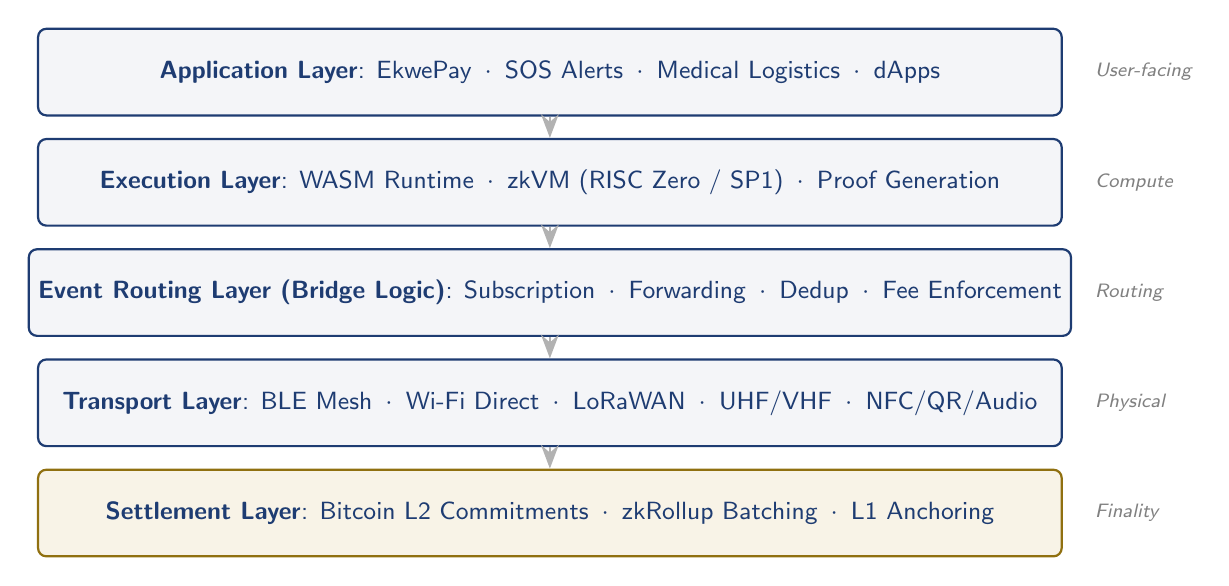
\begin{tikzpicture}[
  layer/.style={
    draw=ekweblue, thick, rounded corners=3pt,
    minimum width=13cm, minimum height=1.1cm,
    fill=ekweblue!5, font=\sffamily\small,
    text=ekweblue
  },
  label/.style={font=\sffamily\scriptsize\itshape, text=gray},
  arrow/.style={-{Stealth[length=3mm]}, thick, gray!60}
]
  \node[layer] (L5) at (0,0) {\textbf{Application Layer}: EkwePay \,$\cdot$\, SOS Alerts \,$\cdot$\, Medical Logistics \,$\cdot$\, dApps};
  \node[layer] (L4) at (0,-1.4) {\textbf{Execution Layer}: WASM Runtime \,$\cdot$\, zkVM (RISC Zero / SP1) \,$\cdot$\, Proof Generation};
  \node[layer] (L3) at (0,-2.8) {\textbf{Event Routing Layer (Bridge Logic)}: Subscription \,$\cdot$\, Forwarding \,$\cdot$\, Dedup \,$\cdot$\, Fee Enforcement};
  \node[layer] (L2) at (0,-4.2) {\textbf{Transport Layer}: BLE Mesh \,$\cdot$\, Wi-Fi Direct \,$\cdot$\, LoRaWAN \,$\cdot$\, UHF/VHF \,$\cdot$\, NFC/QR/Audio};
  \node[layer, fill=ekwegold!10, draw=ekwegold!80!black] (L1) at (0,-5.6) {\textbf{Settlement Layer}: Bitcoin L2 Commitments \,$\cdot$\, zkRollup Batching \,$\cdot$\, L1 Anchoring};

  \draw[arrow] (L5.south) -- (L4.north);
  \draw[arrow] (L4.south) -- (L3.north);
  \draw[arrow] (L3.south) -- (L2.north);
  \draw[arrow] (L2.south) -- (L1.north);

  \node[label, right] at (6.8,0) {User-facing};
  \node[label, right] at (6.8,-1.4) {Compute};
  \node[label, right] at (6.8,-2.8) {Routing};
  \node[label, right] at (6.8,-4.2) {Physical};
  \node[label, right] at (6.8,-5.6) {Finality};
\end{tikzpicture}
\caption{Ekwe Protocol layered architecture.}
\label{fig:architecture}
\end{figure}

\begin{enumerate}[nosep]
  \item \textbf{Application Layer}: mission-critical services including EkwePay (offline payments), SOS emergency alerts, medical logistics, and third-party dApps built on the Ekwe SDK.
  \item \textbf{Execution Layer}: optional deterministic execution of event payloads (WASM modules) and receipt/proof generation via zkVM~\cite{risczero}.
  \item \textbf{Event Routing Layer (Bridge Logic)}: subscription management, forwarding policy, deduplication, fee enforcement, receipt handling, and store-and-forward caching.
  \item \textbf{Transport Layer}: heterogeneous radio adapters (BLE mesh, Wi-Fi P2P, LoRaWAN, and optional legacy interfaces)~\cite{lorawan,bt_mesh,wifi_p2p}.
  \item \textbf{Settlement Layer}: Bitcoin L2 commitments with periodic anchoring and dispute pathways~\cite{sok_btc_l2,bitvm2}.
\end{enumerate}

% ============================================================
% 6. NODE ROLES & IDENTITY
% ============================================================
\section{Node Roles and Identity}

\subsection{Identity Model}

Each node in the Ekwe network possesses:
\begin{itemize}[nosep]
  \item A \textbf{Node ID} in Decentralized Identifier (DID) format.
  \item An \textbf{Ed25519 public/private key pair} for signing and verification.
  \item A \textbf{role designation}: Mobile Node, Relay Node, Execution Node, Commit Node, or Smartbox Node.
  \item \textbf{Message filters}: topics, regions, and tags defining subscription interests.
  \item A \textbf{token balance} for spending gas or receiving rewards.
\end{itemize}

\subsection{Node Types}

\begin{table}[ht]
\centering
\caption{Ekwe Protocol node types and capabilities.}
\label{tab:nodes}
\begin{tabular}{@{}lp{9.5cm}@{}}
\toprule
\textbf{Node Type} & \textbf{Description} \\
\midrule
Mobile Node & Smartphone running an Ekwe Edge Agent; capable of subscribing, sending, and optionally relaying events. First-class participant due to ubiquity and multi-radio support. \\
Light Relay & Phone or embedded device providing short-term message caching and BLE/Wi-Fi forwarding with minimal resource commitment. \\
Full Relay & LoRa+Wi-Fi+ZK capable node providing persistent store-and-forward, consensus participation, and higher QoS guarantees. \\
Execution Node & Authorized to execute event payloads (WASM or zkVM modules) and produce verifiable receipts/proofs. \\
Commit Node & Aggregates receipts and posts state commitments to the Bitcoin L2 and periodically to Bitcoin L1. \\
EkweBox & Purpose-built hardware node: solar/AC powered, multi-radio (LoRa + BLE + Wi-Fi), persistent storage. Designed for permanent community relay infrastructure. \\
Smartbox & Advanced EkweBox variant incorporating Interaction Combinator-based ASIC mining hardware, enabling Bitcoin mining alongside event routing. \\
\bottomrule
\end{tabular}
\end{table}

\subsection{Network Assumptions}
\begin{enumerate}[nosep]
  \item Partitions are common; end-to-end paths cannot be assumed.
  \item Nodes are heterogeneous in power, bandwidth, and availability.
  \item Adversarial behavior is possible (spam floods, selective forwarding, replay).
  \item A subset of nodes periodically gains Internet access, enabling delayed global synchronization.
\end{enumerate}

% ============================================================
% 7. EKWE EVENT LAYER
% ============================================================
\section{Ekwe Event Layer}

\subsection{Event Format}

Ekwe Protocol is specified around a compact, signed event envelope. The canonical representation is shown below; serialization may use CBOR or Protocol Buffers for constrained links, with custom compact encodings for LoRa.

\begin{lstlisting}[caption={Ekwe Event envelope (conceptual schema).}]
EkweEvent := {
  event_id       : UUID,
  version        : uint8,
  timestamp      : ISO8601,
  nonce          : uint64,
  from_node_id   : DID,
  to_address     : Address (unicast | multicast | broadcast),
  topic          : string,
  scope          : ScopeDescriptor,
  ttl            : uint16,
  qos_class      : enum { BEST_EFFORT, RELIABLE, CRITICAL },
  payload_type   : enum { DATA, EXECUTABLE, REFERENCE },
  payload        : bytes (inline or content-addressed ref),
  fee            : { f_fwd, f_cmp, f_str },
  fulfillment_policy : FulfillmentPolicy,
  relay_trace    : [NodeID],
  signature      : Ed25519Signature,
  optional_proof : ZKProof | null,
  optional_receipt_ref : Hash | null
}
\end{lstlisting}

Key design decisions:
\begin{itemize}[nosep]
  \item \texttt{to\_address} supports unicast (node), multicast (group), and scoped broadcast.
  \item \texttt{topic} enables pub/sub-style filtering for push-like delivery.
  \item \texttt{ttl} bounds propagation cost and limits stale relays, analogous to TTL concepts in mesh systems~\cite{bt_mesh}.
  \item \texttt{nonce} and \texttt{event\_id} provide replay resistance and deduplication.
  \item \texttt{fee} fields enable per-event gas accounting (Section~\ref{sec:gas}).
\end{itemize}

\subsection{Addressing and Subscription}

Ekwe supports three addressing modes:
\begin{enumerate}[nosep]
  \item \textbf{Unicast}: direct node addressing using DID-like identifiers.
  \item \textbf{Multicast}: group identifiers (e.g., \texttt{clinic:ward-3}, \texttt{market:zone-2}).
  \item \textbf{Scoped broadcast}: geofenced region codes or transport-local broadcast.
\end{enumerate}

Nodes register subscriptions locally in the Edge Agent. When possible, subscription commitments are published to the L2 for accountability in paid delivery contexts.

\subsection{Dissemination Semantics}

Ekwe adopts DTN-aligned store-and-forward semantics~\cite{rfc4838}. Each relay maintains:
\begin{itemize}[nosep]
  \item A bounded cache of recent \texttt{event\_id} values for deduplication.
  \item A local ``interest table'' derived from neighbor subscriptions and observed demand.
  \item A forwarding policy dependent on \texttt{qos\_class}, TTL, fee sufficiency, and local congestion.
\end{itemize}

\textbf{QoS Classes:}
\begin{itemize}[nosep]
  \item \textbf{Class 0 (Best-effort)}: opportunistic forwarding, minimal redundancy.
  \item \textbf{Class 1 (Reliable)}: replication factor $r > 1$ across diverse next-hops when available.
  \item \textbf{Class 2 (Critical)}: priority scheduling, wider replication, and optional acknowledgment aggregation. Reserved for emergency broadcasts and high-value transactions.
\end{itemize}

% ============================================================
% 8. BRIDGE LOGIC / EDGE AGENT
% ============================================================
\section{Bridge Logic (Ekwe Edge Agent)}

The Edge Agent is the protocol's core runtime: a cross-protocol event router and execution engine running on phones, routers, ESP32/Raspberry Pi boards, and custom EkweBox hardware.

\subsection{Functional Responsibilities}

\begin{enumerate}[nosep]
  \item \textbf{Transport multiplexing}: selecting BLE, Wi-Fi P2P, LoRaWAN, or other bearers depending on link availability and policy~\cite{wifi_p2p}.
  \item \textbf{Event normalization}: mapping transport frames into EkweEvent envelopes.
  \item \textbf{Policy enforcement}: TTL checks, rate limits, subscription filters, minimum fee validation.
  \item \textbf{Cryptographic operations}: Ed25519 signing, verification, and receipt handling.
  \item \textbf{Store-and-forward}: caching with eviction strategies, prioritization, and anti-replay logic.
  \item \textbf{Execution dispatch}: routing executable payloads to authorized Execution Nodes.
\end{enumerate}

\subsection{Convergence Layer Abstraction}

Following DTN convergence-layer separation~\cite{rfc4838}, each transport implements a \texttt{ConvergenceAdapter} interface:

\begin{lstlisting}[caption={Convergence Adapter interface.}]
trait ConvergenceAdapter {
  fn discover_neighbors() -> Vec<NeighborDescriptor>;
  fn link_metrics() -> LinkMetrics;  // bandwidth, energy_cost, reliability
  fn send(event: &EkweEvent, neighbor: &NeighborDescriptor) -> Result;
  fn receive() -> Option<EkweEvent>;
}
\end{lstlisting}

This decouples the event layer from transport details, enabling deployment across diverse radios and hardware platforms.

\subsection{Smartphone Relaying}

Smartphones are first-class relayers due to their ubiquity and multi-radio capabilities. Wi-Fi Direct supports peer-to-peer group formation without an access point, enabling ``pop-up'' high-throughput sync clusters~\cite{wifi_p2p}. BLE and Bluetooth Mesh support local dissemination under low power~\cite{bt_mesh}. LoRaWAN bridges extend range via fixed or semi-fixed relay nodes~\cite{lorawan}. Ekwe uses these primitives to approximate push delivery in the absence of Internet by allowing devices to ``listen'' for relevant topics and addresses locally, receiving events through nearby relays.

% ============================================================
% 9. TRANSPORT LAYER
% ============================================================
\section{Transport Layer}

Ekwe employs a \textbf{transport multiplexer} that provides a unified interface across heterogeneous radio technologies. The multiplexer selects the optimal transport based on availability, link quality, energy budget, and payload characteristics.

\begin{table}[ht]
\centering
\caption{Transport characteristics and use cases.}
\label{tab:transports}
\begin{tabular}{@{}llll@{}}
\toprule
\textbf{Transport} & \textbf{Range} & \textbf{Bandwidth} & \textbf{Primary Use} \\
\midrule
BLE Mesh & $\sim$50m & Low & Proximity sync, local relay \\
Wi-Fi Direct & $\sim$200m & High & Bulk sync, cluster formation \\
LoRaWAN & $\sim$10km & Very Low & Wide-area relay, rural coverage \\
UHF/VHF Radio & $\sim$50km & Very Low & Emergency, extreme offline \\
NFC & Contact & Medium & Device pairing, key exchange \\
QR Codes & Visual & One-shot & Offline payment initiation \\
Audio Tones & $\sim$10m & Minimal & Extreme fallback \\
\bottomrule
\end{tabular}
\end{table}

The architectural separation of small control events (transmitted over long-range, low-throughput LoRaWAN) from bulk synchronization phases (executed opportunistically over Wi-Fi Direct) is a central design hypothesis. This enables efficient resource utilization: payment requests and alerts traverse LoRa links, while proof batches and ledger updates synchronize over high-bandwidth local clusters.

% ============================================================
% 10. GAS & INCENTIVE MODEL
% ============================================================
\section{Gas and Incentive Model}
\label{sec:gas}

\subsection{Rationale}

In open relaying networks, anti-spam and incentive alignment are inseparable. Ekwe adopts a per-event gas model that charges for resource consumption and distributes rewards among fulfillment participants. The gas system is \textit{blind} to message type due to zero-knowledge properties; a payment event and an alert event incur fees based on resource usage, not semantic content.

\subsection{Fee Decomposition}

Inspired by TON's multi-phase fee structure~\cite{ton_whitepaper,ton_fees}, Ekwe decomposes event costs into three components:

\begin{enumerate}[nosep]
  \item \textbf{Forwarding Fee} ($f_{\text{fwd}}$): proportional to payload size, hop count, and QoS class.
  \item \textbf{Compute Fee} ($f_{\text{cmp}}$): paid when an Execution Node runs a payload.
  \item \textbf{Storage Fee} ($f_{\text{str}}$): paid for retaining events/receipts beyond an immediate forwarding window.
\end{enumerate}

\subsection{Sponsorship Model}

Ekwe's primary operational model follows an \textbf{integrator-sponsored gas} pathway:
\begin{itemize}[nosep]
  \item An \textbf{Integrator} (e.g., EkwePay operator, clinic system, logistics platform) prepays or sponsors event gas.
  \item The integrator may recoup costs from end-users at the application layer via microinvoicing.
\end{itemize}

This mirrors centralized push economics (operators pay infrastructure costs) while decentralizing the fulfillment path.

\subsection{Reward Splitting}

Each fulfilled event produces a \texttt{FulfillmentReceipt} listing contributing nodes (ordered by \texttt{relay\_trace} and role). Rewards are split as:

\begin{align}
R_{\text{total}} &= f_{\text{fwd}} + f_{\text{cmp}} + f_{\text{str}} \\
R_{\text{relayer}} &= \alpha \cdot f_{\text{fwd}} \\
R_{\text{executor}} &= \beta \cdot f_{\text{cmp}} \\
R_{\text{committer}} &= \gamma \cdot (f_{\text{fwd}} + f_{\text{cmp}}) \\
R_{\text{storage}} &= \delta \cdot f_{\text{str}}
\end{align}

where $\alpha + \beta + \gamma + \delta = 1$. The parameters $\alpha, \beta, \gamma, \delta$ are governance-controlled, published on-chain, and may be dynamically tuned for network conditions.

% ============================================================
% 11. TOKEN ECONOMICS
% ============================================================
\section{Token Economics}

Ekwe Protocol employs a \textbf{dual-token model} designed to align short-term utility with long-term infrastructure investment.

\subsection{The \$EKWE Utility Token}

\$EKWE serves as the native protocol token for:
\begin{itemize}[nosep]
  \item \textbf{Gas payments}: all event fees are denominated in \$EKWE.
  \item \textbf{Node staking}: nodes stake \$EKWE to signal commitment and participate in higher-trust roles (Execution, Commit).
  \item \textbf{dApp access}: third-party applications pay \$EKWE for protocol integration.
  \item \textbf{Governance}: token-weighted voting on protocol parameters ($\alpha, \beta, \gamma, \delta$, fee floors, QoS policies).
\end{itemize}

\subsection{BTC Mining Rewards}

Smartbox nodes (Section~\ref{sec:hardware}) incorporate specialized mining hardware based on Interaction Combinator architectures, enabling energy-efficient Bitcoin mining alongside event routing. BTC rewards are distributed proportionally based on:
\begin{itemize}[nosep]
  \item Node uptime and availability.
  \item Volume of data relayed and events fulfilled.
  \item Mining hashpower contributed to the pooled mining operation.
\end{itemize}

This dual-token structure creates two distinct value streams: \$EKWE captures protocol-level utility and governance, while BTC mining rewards provide a hard-money incentive for deploying and maintaining physical infrastructure, bridging the DePIN model with Bitcoin's established monetary properties.

% ============================================================
% 12. EXECUTION & VERIFIABLE COMPUTING
% ============================================================
\section{Execution and Verifiable Computing}

\subsection{Executable Events}

Some Ekwe events carry logic (or references to logic) requiring deterministic execution:
\begin{itemize}[nosep]
  \item Validating a payment authorization policy.
  \item Performing risk checks and compliance verification.
  \item Generating state transition witnesses for L2 settlement.
  \item Executing smart contract logic at the edge.
\end{itemize}

\subsection{Proof of Execution via zkVM}

Ekwe targets proof-carrying execution using a zero-knowledge virtual machine (zkVM). RISC Zero provides receipts that prove correct execution of arbitrary code without revealing additional information beyond what is encoded in the receipt~\cite{risczero}. Ekwe's Execution Nodes generate proofs/receipts that are:
\begin{enumerate}[nosep]
  \item Locally verifiable by nearby nodes (where feasible).
  \item Batch-committable to the L2 for dispute resolution.
\end{enumerate}

In bandwidth-constrained settings, receipts may be generated asynchronously and propagated as follow-on events, allowing dissemination and settlement to proceed even when proof generation is delayed.

\subsection{Execution Runtimes}

The protocol supports multiple execution backends:
\begin{itemize}[nosep]
  \item \textbf{WASM}: lightweight, portable execution for general event payloads.
  \item \textbf{zkVM (RISC Zero, SP1)}: for high-assurance proofs on critical operations~\cite{risczero}.
  \item \textbf{zkWASM}: combining WASM portability with zero-knowledge proof generation.
  \item \textbf{Rules Engine}: a rule-based router for simple event processing and cache-first logic on resource-constrained nodes.
\end{itemize}

% ============================================================
% 13. BITCOIN L2 ANCHORING & SETTLEMENT
% ============================================================
\section{Bitcoin L2 Anchoring and Settlement}

\subsection{Design Positioning}

Bitcoin L2 systems vary widely; a recent Systematization of Knowledge identifies multiple design patterns for constructing L2s via transaction modifications and proof mechanisms~\cite{sok_btc_l2}. Ekwe adopts a pattern compatible with:
\begin{enumerate}[nosep]
  \item Periodic commitments to Bitcoin for auditability.
  \item L2 dispute framing that can tolerate delayed connectivity.
\end{enumerate}

\subsection{Bridging and Dispute Framing}

BitVM2 proposes a paradigm for enabling arbitrary program verification using Bitcoin as a dispute layer, including a bridge design for L2 systems~\cite{bitvm2}. Ekwe's roadmap is compatible with BitVM-style challenge mechanisms for:
\begin{itemize}[nosep]
  \item Bridging BTC into the Ekwe L2.
  \item Enforcing settlement outcomes for disputed transactions.
  \item Verifying execution receipts on-chain when challenged.
\end{itemize}

\subsection{Settlement for EkwePay}

EkwePay requires a clear separation between:
\begin{enumerate}[nosep]
  \item \textbf{Local authorization}: user experience under outage, with signed intents and bounded validity windows.
  \item \textbf{Eventual settlement}: final ledger updates anchored to the L2 and periodically to Bitcoin L1 upon synchronization.
\end{enumerate}

The protocol treats offline approvals as signed intents with bounded validity windows and risk controls, with final ledger updates occurring upon any node regaining backhaul connectivity.

\subsection{Chain Design Options}

Ekwe's settlement layer is designed to be modular:
\begin{itemize}[nosep]
  \item \textbf{zkRollup}: batched proofs from Execution Nodes committed to Bitcoin L2.
  \item \textbf{DAG with lazy finality}: lightweight consensus for edge environments.
  \item \textbf{Federation}: initial bootstrap mechanism for early network deployment.
  \item \textbf{Embedded mini-chain}: local SQLite-based chain or zk-rollup buffer for offline operation.
\end{itemize}

% ============================================================
% 14. EKWEPAY FLAGSHIP USE CASE
% ============================================================
\section{EkwePay: Flagship Use Case}

EkwePay is the flagship application demonstrating Ekwe Protocol's capabilities for offline-first financial transactions. It differs from USSD-based mobile money in two fundamental ways: (I)~USSD requires cellular service continuity~\cite{etsi_ussd_stage1}; (II)~EkwePay operates over community-provisioned local transports with eventual settlement.

\subsection{Transaction Workflow}

Figure~\ref{fig:ekwepay} illustrates the complete EkwePay transaction flow.

\begin{figure}[ht]
\centering
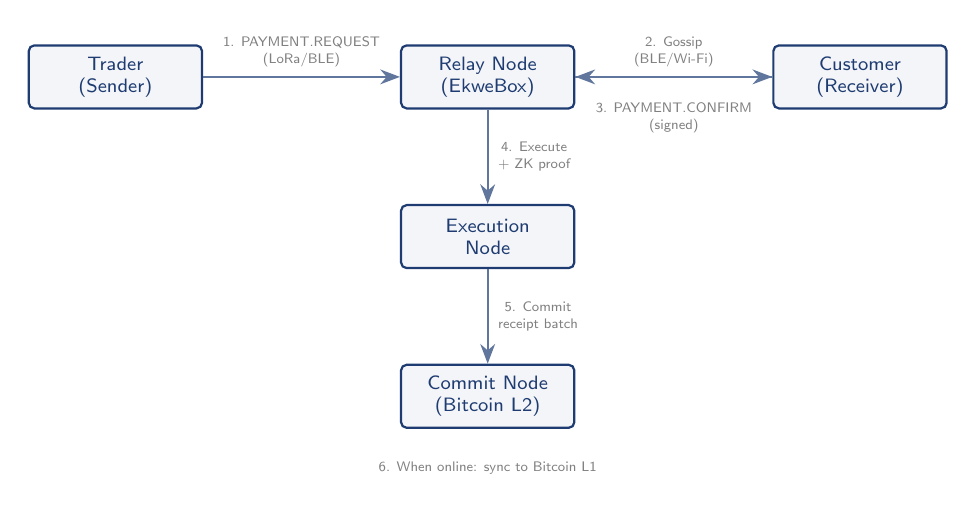
\begin{tikzpicture}[
  node distance=0.6cm and 2cm,
  box/.style={draw=ekweblue, thick, rounded corners=2pt, minimum width=2.2cm, minimum height=0.8cm, fill=ekweblue!5, font=\sffamily\scriptsize, text=ekweblue, align=center},
  arrow/.style={-{Stealth[length=2.5mm]}, thick, ekweblue!70},
  label/.style={font=\sffamily\tiny, text=gray, align=center}
]
  \node[box] (trader) {Trader\\(Sender)};
  \node[box, right=2.5cm of trader] (relay1) {Relay Node\\(EkweBox)};
  \node[box, right=2.5cm of relay1] (customer) {Customer\\(Receiver)};
  \node[box, below=1.2cm of relay1] (executor) {Execution\\Node};
  \node[box, below=1.2cm of executor] (chain) {Commit Node\\(Bitcoin L2)};

  \draw[arrow] (trader) -- node[above, label] {1. PAYMENT.REQUEST\\(LoRa/BLE)} (relay1);
  \draw[arrow] (relay1) -- node[above, label] {2. Gossip\\(BLE/Wi-Fi)} (customer);
  \draw[arrow] (customer) -- node[below, label, yshift=-2mm] {3. PAYMENT.CONFIRM\\(signed)} (relay1);
  \draw[arrow] (relay1) -- node[right, label] {4. Execute\\+ ZK proof} (executor);
  \draw[arrow] (executor) -- node[right, label] {5. Commit\\receipt batch} (chain);

  \node[label, below=0.3cm of chain] {6. When online: sync to Bitcoin L1};
\end{tikzpicture}
\caption{EkwePay offline transaction workflow.}
\label{fig:ekwepay}
\end{figure}

\textbf{Detailed steps:}
\begin{enumerate}[nosep]
  \item \textbf{Initiation}: Trader creates a \texttt{PAYMENT.REQUEST} event on her phone (e.g., \texttt{\{amount: 2500, currency: ``NGN''\}}).
  \item \textbf{Relay}: Nearby EkweBox gossips the event over LoRa; other nodes forward via BLE/Wi-Fi.
  \item \textbf{Delivery}: Customer's phone receives the request via BLE from a nearby relay.
  \item \textbf{Confirmation}: Customer signs a \texttt{PAYMENT.CONFIRM} event, relayed back through the network.
  \item \textbf{Execution}: An Execution Node validates the authorization, runs payment logic (WASM/zkVM), generates a proof, and queues a commitment.
  \item \textbf{Settlement}: When any node regains Internet, proofs and receipts are batch-committed to the Bitcoin L2.
  \item \textbf{Gas distribution}: Fees are split among the trader's integrator (originator), all relayers in the trace, the executor, and the commit node.
\end{enumerate}

\subsection{Offline Risk Controls}

To control offline risk, EkwePay policies include:
\begin{itemize}[nosep]
  \item \textbf{Bounded transaction limits}: maximum offline transaction value per identity per time window.
  \item \textbf{Short validity windows}: signed intents expire, preventing indefinite deferral.
  \item \textbf{Delayed finality}: transactions are provisional until settlement confirmation.
  \item \textbf{Reputation staking}: nodes and users stake \$EKWE against misbehavior.
\end{itemize}

% ============================================================
% 15. HARDWARE: EKWEBOX / SMARTBOX
% ============================================================
\section{Hardware: EkweBox and Smartbox}
\label{sec:hardware}

\subsection{EkweBox}

The EkweBox is purpose-built hardware designed for permanent community relay infrastructure:
\begin{itemize}[nosep]
  \item \textbf{Radios}: LoRa transceiver + BLE 5.0 + Wi-Fi (AP + P2P mode).
  \item \textbf{Compute}: ARM-based SoC (e.g., Raspberry Pi CM4 or ESP32-S3 for lower cost).
  \item \textbf{Storage}: Local flash/SD for event cache and partial blockchain state.
  \item \textbf{Power}: Solar panel + battery + optional AC, designed for 24/7 operation in off-grid environments.
  \item \textbf{Interface}: USB/Serial for integration; optional display for diagnostics.
\end{itemize}

\subsection{Smartbox}

The Smartbox extends the EkweBox with mining capabilities:
\begin{itemize}[nosep]
  \item All EkweBox capabilities, plus:
  \item \textbf{Mining ASIC}: Interaction Combinator-based ASIC architecture for energy-efficient Bitcoin mining.
  \item \textbf{ZK co-processor}: hardware acceleration for proof generation.
  \item \textbf{Enhanced storage}: for archival node functionality and full blockchain state.
\end{itemize}

The Smartbox creates a compelling DePIN value proposition: a single device routes Ekwe events (earning \$EKWE gas fees), mines Bitcoin (earning BTC), and provides community communication infrastructure, all powered by solar energy.

% ============================================================
% 16. SECURITY & PRIVACY
% ============================================================
\section{Security and Privacy}

\subsection{Identity and Authentication}
Nodes are bound to Ed25519 cryptographic identities. All events are signed at origin and verified at each relay and execution hop. Local user authentication employs JWT or passcode-based mechanisms.

\subsection{Replay, Spam, and Flooding Resistance}
\begin{itemize}[nosep]
  \item \textbf{Replay resistance}: event identifiers, monotonic nonces, and bounded TTL.
  \item \textbf{Spam resistance}: minimum fee policies and rate limits at relays; higher QoS classes require stronger fee commitments.
  \item \textbf{Anti-flooding}: TTL bounds prevent indefinite message propagation.
\end{itemize}

\subsection{Sybil Resistance}
Fee-only resistance is insufficient in adversarial environments. Ekwe employs a layered approach:
\begin{itemize}[nosep]
  \item \textbf{Stake requirements}: nodes must stake \$EKWE proportional to their role privileges.
  \item \textbf{Proof-of-availability}: tracked uptime and relay metrics.
  \item \textbf{Reputation signals}: historical fulfillment accuracy.
  \item \textbf{Governance thresholds}: dynamically adjusted based on network conditions.
\end{itemize}

\subsection{Privacy and Metadata Minimization}
Relay traces support reward attribution but introduce metadata leakage risks. Ekwe treats privacy-preserving accounting as a first-class design concern:
\begin{itemize}[nosep]
  \item \textbf{ZK-based reward claims}: proving relay participation without revealing the full trace.
  \item \textbf{Blinded relay sets}: aggregated receipts that obscure individual node contributions.
  \item \textbf{End-to-end encryption}: event payloads are encrypted; only addressing metadata is visible to relays.
  \item \textbf{Gas blindness}: fees are computed on resource usage, not message content, due to ZK properties.
\end{itemize}

% ============================================================
% 17. IMPLEMENTATION BLUEPRINT & EVALUATION
% ============================================================
\section{Implementation Blueprint and Evaluation Methodology}

\subsection{Reference Implementation}

\begin{table}[ht]
\centering
\caption{Implementation components.}
\label{tab:impl}
\begin{tabular}{@{}llp{6.5cm}@{}}
\toprule
\textbf{Component} & \textbf{Technology} & \textbf{Description} \\
\midrule
Edge Agent & Rust/Go & Cross-platform, embeddable runtime with event store, verifier, forwarder, and subscription manager \\
Mobile App & Flutter + Native SDK & Runs Edge Agent; provides UX for EkwePay, contact book, QR sync \\
Radio Stack & Hardware APIs & LoRaWAN (Semtech), BLE (ESP32/phone), Wi-Fi Direct \\
Execution VM & WASM / zkVM & Deterministic execution with receipt generation~\cite{risczero} \\
Mini-Chain & Embedded DB & SQLite-based local chain or zk-rollup buffer \\
Rules Engine & Embedded & Rule-based event router for cache-first logic \\
\bottomrule
\end{tabular}
\end{table}

\subsection{Evaluation Metrics}
\begin{enumerate}[nosep]
  \item \textbf{Delivery ratio}: fraction of targeted nodes receiving an event within time $T$.
  \item \textbf{Latency distribution}: end-to-end time under partitioned mobility.
  \item \textbf{Overhead}: transmissions per delivered event (by transport and QoS class).
  \item \textbf{Energy proxy}: radio-on time and bytes transmitted by role.
  \item \textbf{Economic efficiency}: reward per delivered byte and spam cost.
\end{enumerate}

\subsection{Evaluation Scenarios}
\begin{enumerate}[nosep]
  \item \textbf{Rural partition}: simulated villages with sparse nodes and intermittent backhaul; compare QoS classes and replication factors.
  \item \textbf{Urban congestion}: high node density with adversarial spam; evaluate fee-based throttling.
  \item \textbf{Mixed-transport}: BLE/Wi-Fi clusters bridged by LoRaWAN relays; quantify cross-transport propagation.
\end{enumerate}

\subsection{Baselines}
\begin{enumerate}[nosep]
  \item \textbf{Centralized push}: APNs/FCM delivery degrades to zero without Internet~\cite{apns}.
  \item \textbf{DTN baseline}: store-and-forward overlay without incentives~\cite{rfc4838}.
  \item \textbf{DePIN coverage}: incentive-driven coverage (Helium-style) without general event execution~\cite{helium}.
\end{enumerate}

% ============================================================
% 18. ROADMAP
% ============================================================
\section{Roadmap}

\begin{table}[ht]
\centering
\caption{Ekwe Protocol development roadmap.}
\label{tab:roadmap}
\begin{tabular}{@{}llp{8cm}@{}}
\toprule
\textbf{Phase} & \textbf{Version} & \textbf{Milestones} \\
\midrule
Foundation & v0.1 & System design document; core protocol specification; Edge Agent prototype (Rust) \\
Tokenomics & v0.2 & \$EKWE token design; staking model; gas parameter calibration \\
Hardware & v0.3 & EkweBox hardware specification; Smartbox design with Interaction Combinator ASIC integration \\
Developer & v0.4 & App SDKs (Android/iOS); developer portal; third-party dApp integration APIs \\
Testnet & v0.5 & Public testnet; controlled rural and urban pilot deployments \\
Mainnet & v1.0 & Production-ready zk-Execution engine; Bitcoin L2 rollup chain; EkwePay launch \\
Scale & v2.0 & Multi-region sync bridges; priority emergency lanes; cross-chain interoperability \\
\bottomrule
\end{tabular}
\end{table}

% ============================================================
% 19. LIMITATIONS & OPEN PROBLEMS
% ============================================================
\section{Limitations and Open Problems}

\begin{enumerate}[nosep]
  \item \textbf{Offline double-spend}: purely offline payments require careful risk bounding (limits, time windows, and eventual settlement). Fully offline double-spend prevention for high-value payments remains outside scope without additional synchronization or trusted hardware assumptions.
  \item \textbf{Sybil resistance}: permissionless relaying needs robust anti-Sybil mechanisms beyond fees alone (stake, proof-of-coverage, reputation). The optimal combination remains an empirical question.
  \item \textbf{Privacy vs.\ accountability}: relay traces aid reward splitting but can leak metadata; privacy-preserving accounting (ZK-based reward claims, blinded relay sets) remains an active research direction.
  \item \textbf{Mobile OS constraints}: background relaying is limited by platform policies (iOS background execution, Android Doze mode); dedicated Smartboxes are required for high-availability deployments.
  \item \textbf{Governance calibration}: fee parameters ($\alpha, \beta, \gamma, \delta$) and reward splits require empirical tuning under real deployment conditions.
  \item \textbf{Consensus finalization}: the optimal consensus mechanism for challenged-network environments with intermittent global synchronization remains an open design question.
\end{enumerate}

% ============================================================
% 20. CONCLUSION
% ============================================================
\section{Conclusion}

Ekwe Protocol is specified as a decentralized, event-driven edge substrate that generalizes ``push notifications'' into a resilient, offline-first dissemination and execution layer. Drawing inspiration from the Igbo Ekwe drum, a community-operated, decentralized communication instrument, the protocol reimagines critical infrastructure for environments where connectivity cannot be assumed.

The protocol differs from centralized push systems by removing dependence on always-on Internet brokers, and it differs from USSD-based financial access by enabling operation beyond the operator signaling plane, including scenarios where cellular coverage is absent or unreliable~\cite{apns,etsi_ussd_stage1}. Ekwe integrates DTN-style store-and-forward routing~\cite{rfc4838}, multi-radio relaying across BLE, Wi-Fi Direct, and LoRaWAN~\cite{bt_mesh,wifi_p2p,lorawan}, TON-inspired gas accounting with reward splitting~\cite{ton_whitepaper,ton_fees}, verifiable execution via zkVM~\cite{risczero}, and Bitcoin L2 anchoring for settlement~\cite{sok_btc_l2,bitvm2}.

The dual-token model (\$EKWE for protocol utility and BTC from Smartbox mining) creates aligned incentives for deploying and maintaining physical infrastructure. The flagship application, EkwePay, demonstrates how offline-first financial transactions can operate through community-provisioned relay networks with eventual settlement on Bitcoin.

The next research and engineering steps include: a reference implementation of the Edge Agent; controlled evaluation across rural and urban deployment scenarios; formalization of privacy-preserving incentive accounting; and production of the EkweBox and Smartbox hardware platforms.

\vspace{0.5cm}
\noindent\textit{The drum speaks. The network listens. The people are sovereign.}

% ============================================================
% REFERENCES
% ============================================================
\begin{thebibliography}{20}

\bibitem{rfc4838}
V.~Cerf \textit{et al.}, ``Delay-Tolerant Networking Architecture,'' RFC~4838, IETF, 2007. [Online]. Available: \url{https://www.rfc-editor.org/rfc/rfc4838.html}

\bibitem{apns}
Apple Developer Documentation, ``Establishing a Token-Based Connection to APNs,'' Apple Push Notification service. [Online]. Available: \url{https://developer.apple.com/documentation/usernotifications/establishing-a-token-based-connection-to-apns}

\bibitem{fcm}
Google Firebase Documentation, ``Send a Message Using the FCM HTTP v1 API,'' Firebase Cloud Messaging. [Online]. Available: \url{https://firebase.google.com/docs/cloud-messaging/send/v1-api}

\bibitem{etsi_ussd_stage1}
ETSI (3GPP), ``TS~122~090: Unstructured Supplementary Service Data (USSD); Stage~1,'' v18.0.1. [Online]. Available: \url{https://www.etsi.org/deliver/etsi_ts/122000_122099/122090/18.00.01_60/ts_122090v180001p.pdf}

\bibitem{etsi_ussd_stage2}
ETSI (3GPP), ``TS~123~090: Unstructured Supplementary Service Data (USSD); Stage~2,'' v7.0.0. [Online]. Available: \url{https://www.etsi.org/deliver/etsi_ts/123000_123099/123090/07.00.00_60/ts_123090v070000p.pdf}

\bibitem{gsma_ussd}
GSMA, ``Beyond USSD: How Offline NFC Transactions Can Drive Mobile Money Use,'' 2025. [Online]. Available: \url{https://www.gsma.com/solutions-and-impact/connectivity-for-good/mobile-for-development/blog/beyond-ussd-how-offline-nfc-transactions-can-drive-mobile-money-use/}

\bibitem{lorawan}
LoRa Alliance, ``TS001-1.0.4 LoRaWAN\textsuperscript{\textregistered} L2 1.0.4 Specification,'' 2023. [Online]. Available: \url{https://resources.lora-alliance.org/technical-specifications/ts001-1-0-4-lorawan-l2-1-0-4-specification}

\bibitem{bt_mesh}
Bluetooth SIG, ``Bluetooth Mesh Profile 1.0.1,'' Adopted Specification. [Online]. Available: \url{https://www.bluetooth.com/specifications/specs/mesh-profile-1-0-1/}

\bibitem{wifi_p2p}
Android Developers, ``Wi-Fi Direct (Wi-Fi P2P) Overview.'' [Online]. Available: \url{https://developer.android.com/develop/connectivity/wifi/wifip2p}

\bibitem{ton_whitepaper}
The Open Network (TON), ``TON Whitepaper,'' 2021. [Online]. Available: \url{https://ton.org/whitepaper.pdf}

\bibitem{ton_fees}
TON Documentation, ``Transaction Fees.'' [Online]. Available: \url{https://docs.ton.org/foundations/fees}

\bibitem{sok_btc_l2}
M.~Qi \textit{et al.}, ``SoK: Bitcoin Layer Two (L2),'' \textit{ACM Computing Surveys}, 2025. [Online]. Available: \url{https://dl.acm.org/doi/10.1145/3763232}

\bibitem{bitvm2}
R.~Linus, ``BitVM2: Bridging Bitcoin to Second Layers,'' 2024. [Online]. Available: \url{https://bitvm.org/bitvm_bridge.pdf}

\bibitem{risczero}
RISC Zero, ``Proof System Overview,'' Developer Documentation. [Online]. Available: \url{https://dev.risczero.com/proof-system/}

\bibitem{helium}
Helium, ``Helium Whitepaper.'' [Online]. Available: \url{https://whitepaper.helium.com/}

\bibitem{messari_depin}
Messari, ``Understanding DePIN,'' 2023--2024. [Online]. Available: \url{https://messari.io/copilot/share/understanding-depin-26867bfa-d608-49bf-a2c3-0f14d76f2d6a}

\end{thebibliography}

\end{document}
